\subsection{Operational Mechanism of Solid-State Drives (SSD)}
Unlike HDDs, SSDs perform all storage operations electronically without moving components\cite{gfg_disk_mgmt}.

\begin{enumerate}[label=\roman*.]

    \item Data Writing
    When the operating system sends data, the SSD controller determines suitable NAND flash blocks and
    programs electrical charges into memory cells\cite{openai2026nvmearchitecture}.

    \item  Data Reading
    During read operations, the controller measures the electrical charge stored in each memory cell and converts
    it into digital information\cite{openai2026nvmearchitecture}.

    \item  Flash Translation Layer (FTL)
    The Flash Translation Layer maps logical block addresses provided by the operating system to physical
    locations within NAND flash memory, allowing transparent storage management \cite{lexar_nvme, openai2026nvmearchitecture}.

    \item Background Maintenance
    The SSD controller continuously performs garbage collection, bad block management, wear leveling, and error
    correction to maintain performance and reliability\cite{lexar_nvme}.

\end{enumerate}

\subsubsection{SSD Form Factors}

\begin{enumerate}[label=\roman*.]
    \item  2.5-inch SATA SSD
    The most common SSD form factor for desktops and laptops. It uses the SATA interface and typically provides
    transfer speeds up to approximately 550 MB/s\cite{gfg_storage_structure}.
    
    \item M.2 SATA SSD
    A compact SSD designed primarily for modern laptops and small-form-factor computers. Although physically
    smaller, it still communicates using the SATA interface\cite{lexar_nvme}.
    
    
    \item  mSATA SSD
    An older compact SSD standard used in Ultrabook and embedded systems. It has largely been replaced by M.2
    SSDs\cite{gfg_storage_structure}.
    \item Enterprise SSDs
    Enterprise-grade SSDs are designed for servers and data centers, providing higher endurance, reliability, and
    continuous 24/7 operation\cite{gfg_disk_mgmt}.
\end{enumerate}


\begin{figure}[H]
    \centering

    \begin{subfigure}{0.3\textwidth}
        \centering
        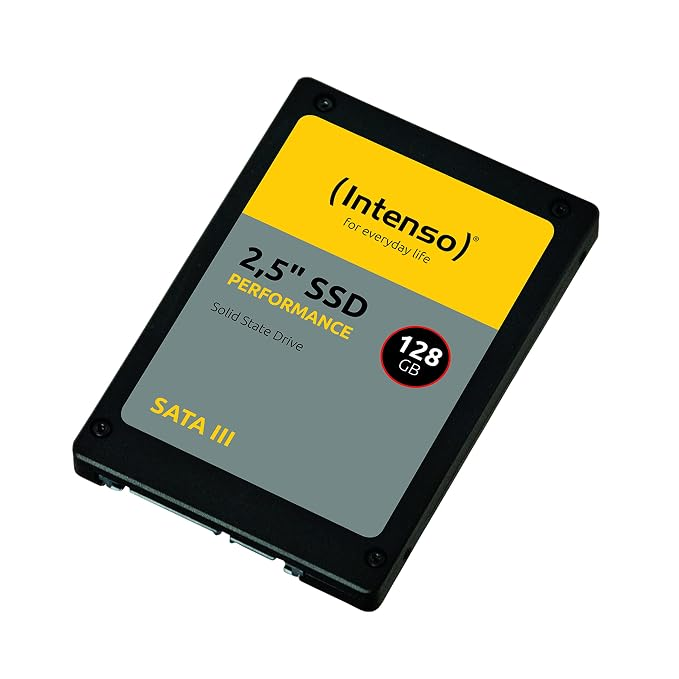
\includegraphics[width=\linewidth]{2.5_SSD.jpg}
        \caption{2.5 SATA SSD\cite{intenso_ssd_amazon}}
    \end{subfigure}
    \hfill
    \begin{subfigure}{0.3\textwidth}
        \centering
        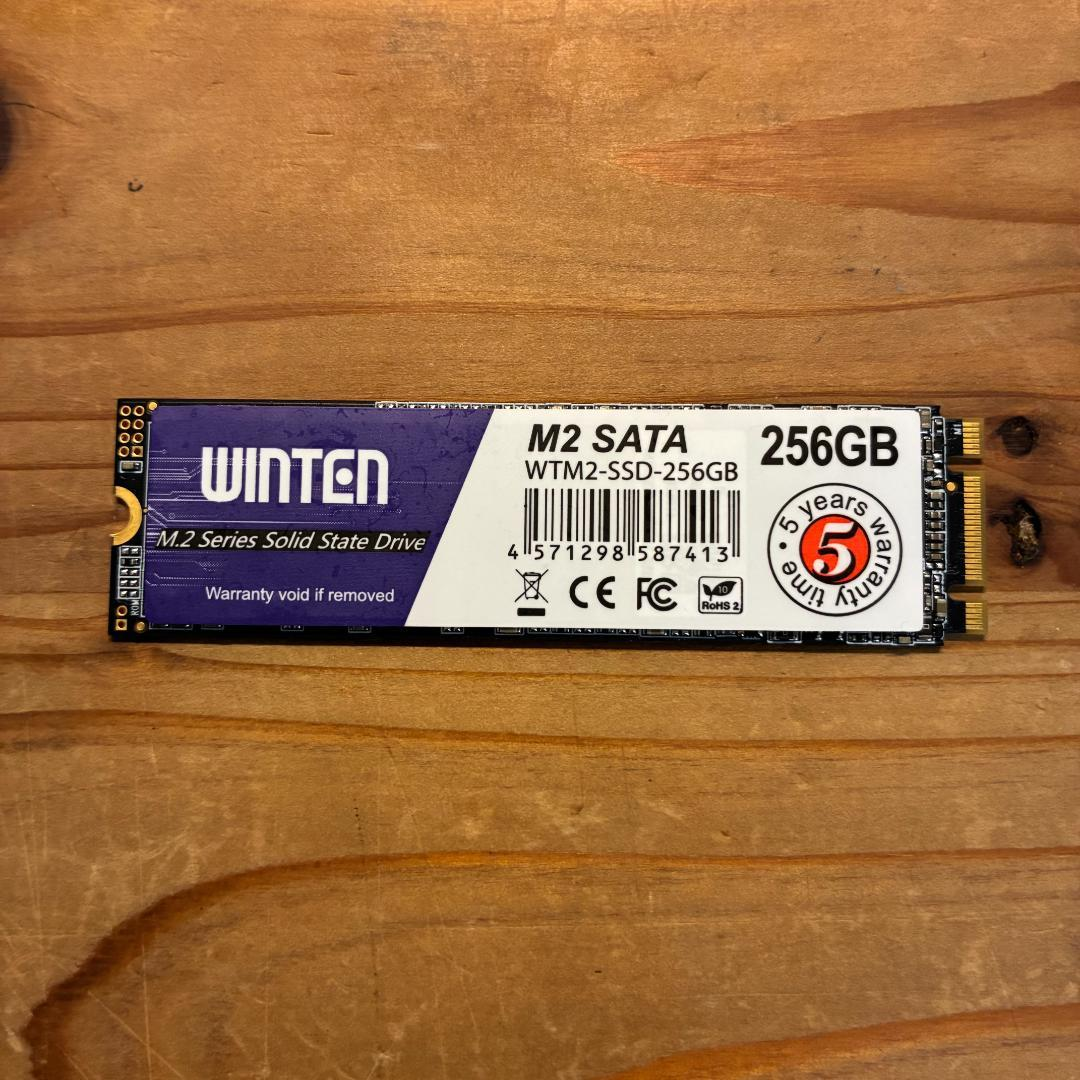
\includegraphics[width=\linewidth]{M2-SATA_SSD.jpg}
        \caption{M.2 SATA SSD\cite{winten_ssd_mercari}}
    \end{subfigure}
    \hfill
    \begin{subfigure}{0.3\textwidth}
        \centering
        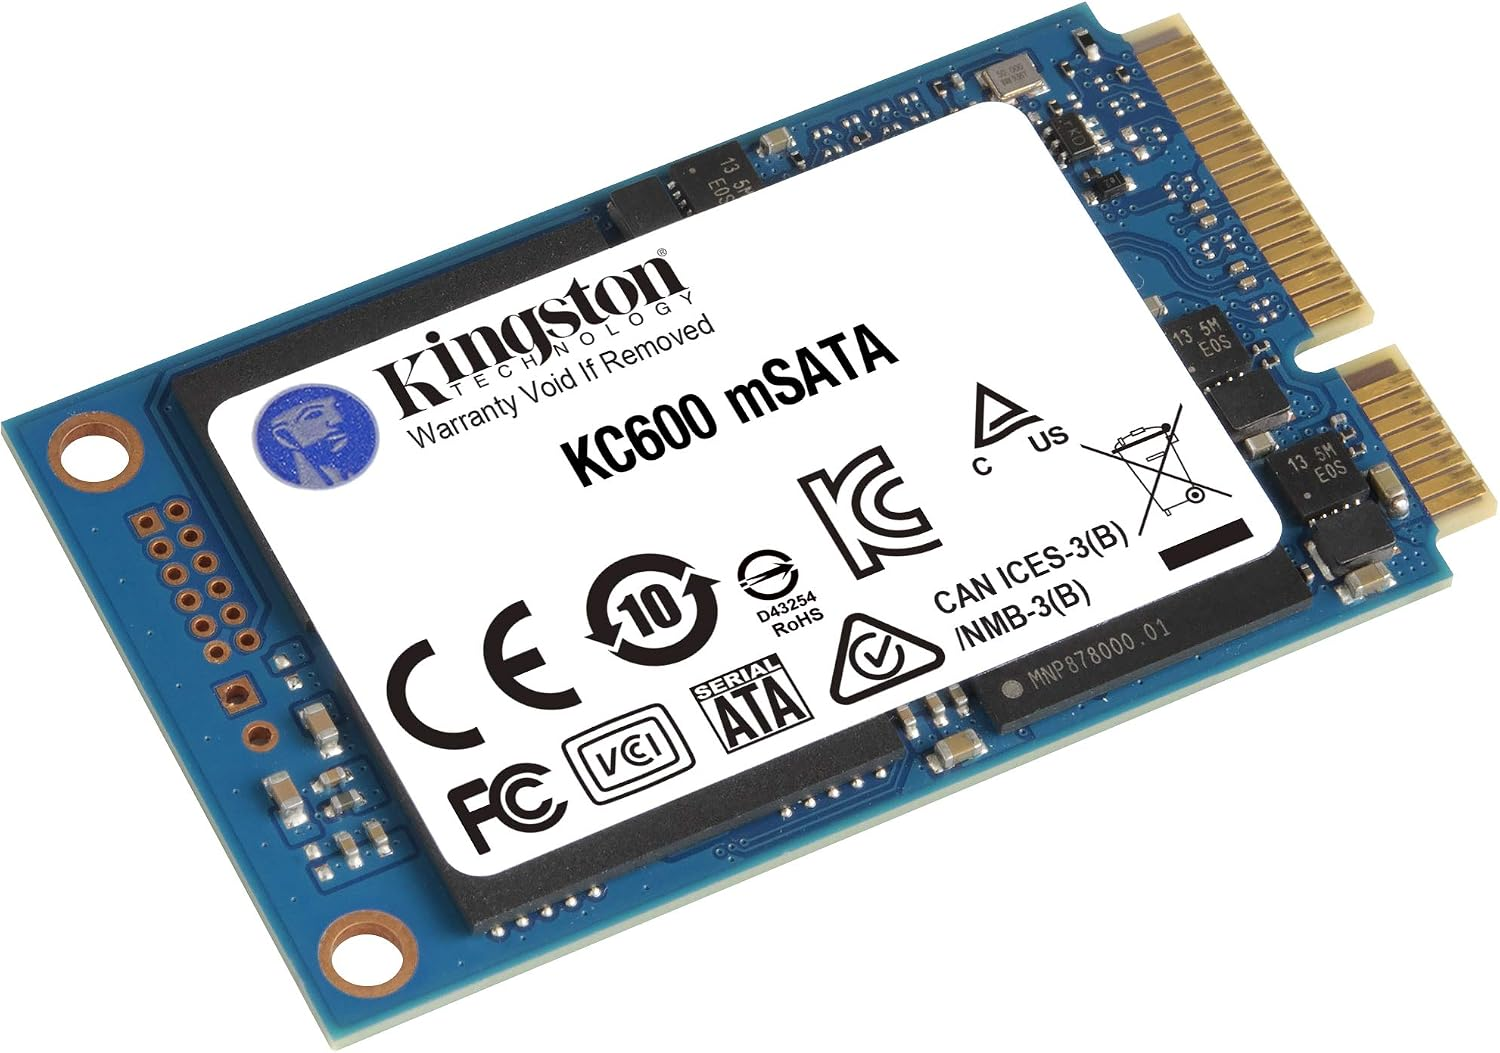
\includegraphics[width=\linewidth]{3m_SATA.jpg}
        \caption{3m SATA SSD\cite{kingston_kc600_amazon}}
    \end{subfigure}

    \caption{Common SATA SSD Form Factors}
    \label{fig:sata_ssd_ff}
\end{figure}


